\chapter{Access to Finance}

\section*{Number of people with access to financial services as a result of DFID support.}


\thispagestyle{empty}


\section{Results}



Between 2015 and 2019 DFID supported \textbf{69.2} million people to gain access to finance, including 35.4 million women, representing 51\% of the total. %

From 2015 to 2019, the largest number of people supported by DFID programmes were in Asia, with 41.3 million people supported (Figure \ref{fig:a2f_region_plot}). In Africa, DFID supported 26.8 million people, in the Middle East 0.9 million people were supported and 0.01 million people were supported through centrally managed programmes. %


\begin{figure}[htbp]
  \centering
\begin{knitrout}
\definecolor{shadecolor}{rgb}{0.969, 0.969, 0.969}\color{fgcolor}
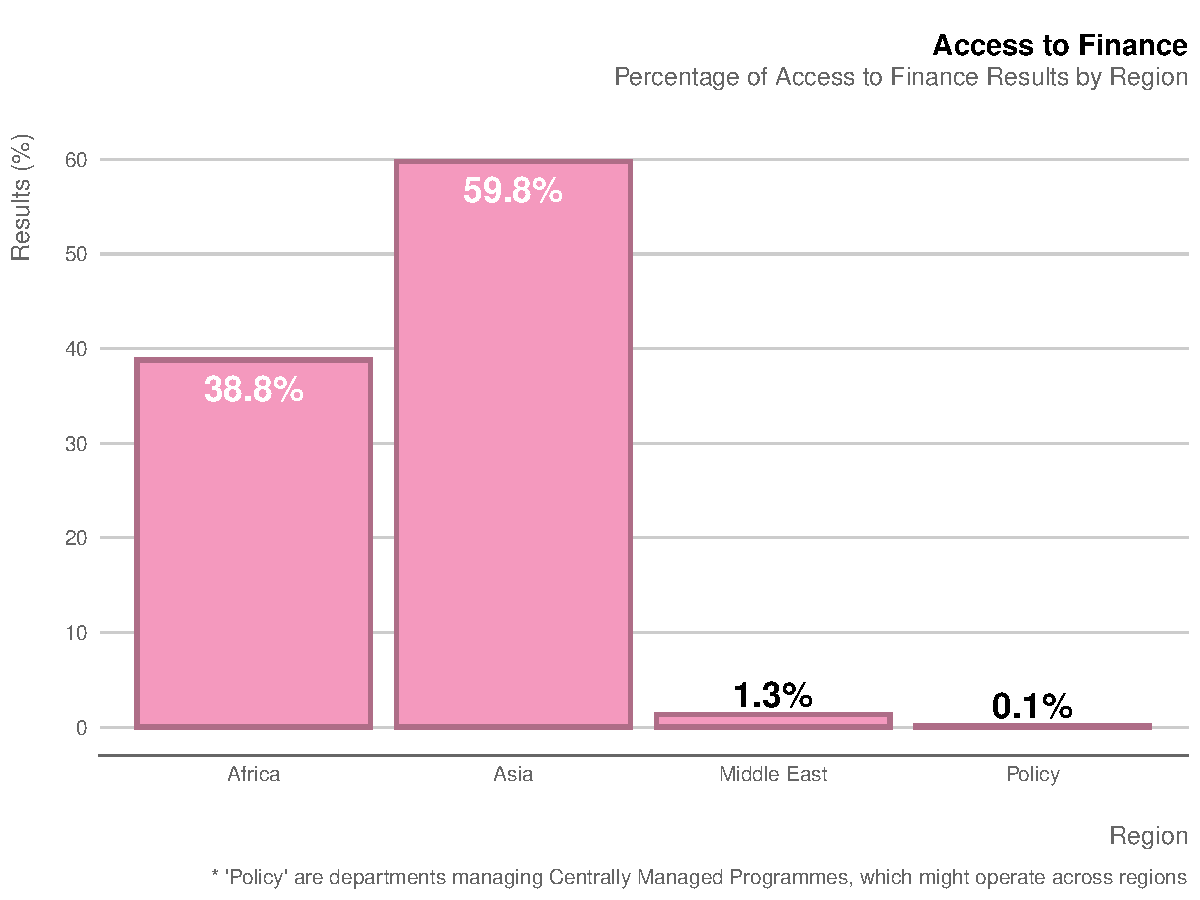
\includegraphics[width=0.8\textwidth]{figs/a2f_region_plot-1} 

\end{knitrout}
%	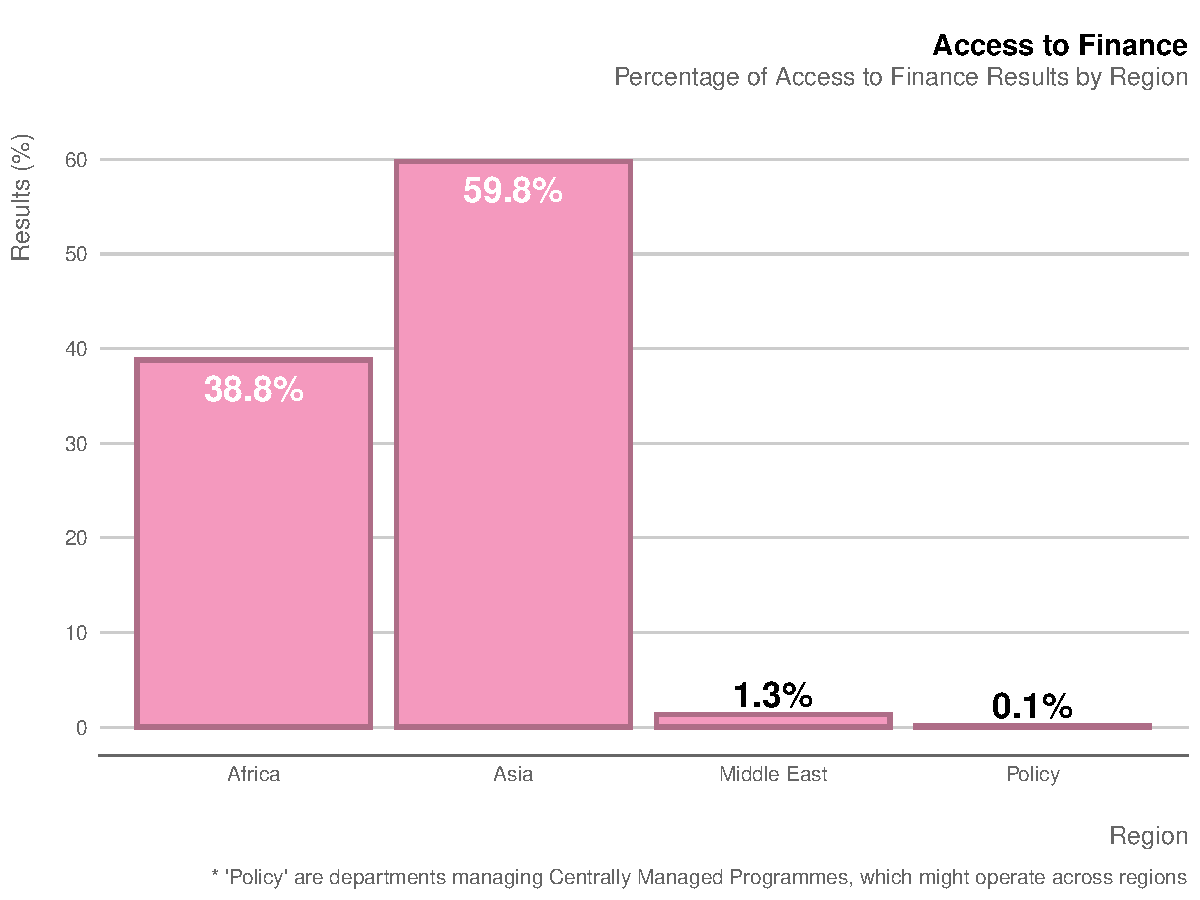
\includegraphics[width=0.8\textwidth]{../figs/a2f_region_plot} \hfill
	\caption{Percentage of Access to Finance results by region.}
	\label{fig:a2f_region_plot}
\end{figure}

\section{Context}
DFID's Economic Development Strategy aims to `improve access to finance for both poor women and men,
helping them to generate and protect their own wealth.' %
This includes supporting improved access to financial services such as secure savings, money transfer, insurance and affordable loans. %

Access to financial services is expected to enhance the welfare of poor households by helping them to
smooth consumption, invest in enterprise, save and become more resilient to all kinds of economic, social
and environmental shocks, send and receive remittances (potentially with less associated costs) and
access credit if and when needed e.g. through access to affordable mortgages. %

DFID support in this area ensures that basic financial services are provided, there is facilitation of businesses growth and job creation, and that people are given support to better manage their own lives and help to escape poverty. %

\newpage
